\documentclass[catalan, a4paper, nobib]{tufte-handout}

% encoding
\usepackage[utf8]{inputenc}
\usepackage[T1]{fontenc}
\usepackage{lmodern}
\usepackage{babel}

\frenchspacing
\usepackage[style=spanish]{csquotes}
\MakeAutoQuote{«}{»}

\usepackage{booktabs}
\usepackage{circuitikz}
\usepackage{siunitx}
\usepackage{amsmath}

\graphicspath{
    {fotos/}
}

% hyperlink setup / metadata
\usepackage{hyperref}
\AfterPreamble{\hypersetup{
  %%pdfauthor={},
  %%pdftitle={},
  %%pdfsubject={},
}}

% document metadata
\author{Víctor Méndez}
\title{ICOM: Pràctica 1}
\date{28-2-2024}

\begin{document}

\maketitle

\newthought{Activitat 1.1} De fet, el senyal que surt pel SA té una potència de \qty[qualifier-mode = combine]{-4.5}{\deci\bel\of{m}}. El GF ha duplicat l'amplitud de sortida per tal que a la resistència càrrega (el SA) es mesuri l'amplitud desitjada; això explica la disparitat entre el valor calculat a la qüestió 1.2 i la mesura. El mesclador és una transformació puntual i no lineal, per aquest motiu s'observen harmònics no desitjats.

\newthought{Activitat 1.2} Veure figura \ref{fig:q1}.

\begin{description}
    \item[Ref] Correspon a la potència observable més alta.
    \item[Att] El factor d'atenuació de l'entrada (pel bon funcionament del mesclador).
    \item[RBW] L'ample de banda del filtre estàtic. La resolució en freqüència depén d'aquest factor.
    \item[VBW] L'ample de banda del filtre passa-baix que es passa a l'hora de mostrar el senyal per pantalla.
    \item[SWT] El temps que triga en fer un escombrat i actualitzar la pantalla.
    \item[Trig] El mode de trigger, igual que en un osci\l.oscopi.
    \item[Center] La freqüència central que es mostra per pantalla.
    \item[Span] L'ample de banda que es mostra per pantalla.
\end{description}

\begin{figure}
    \begin{center}
        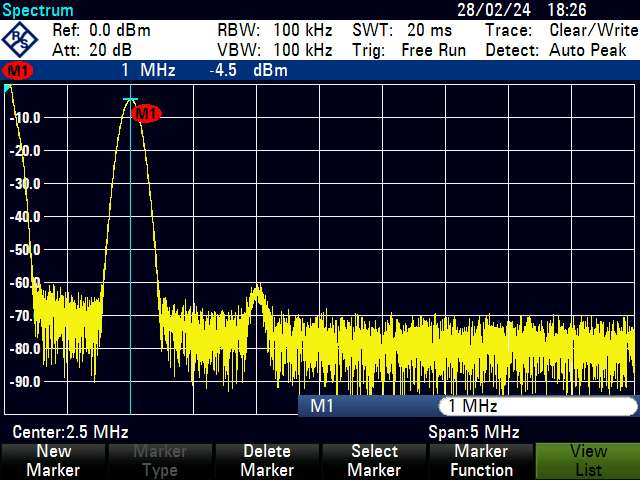
\includegraphics[width=292px]{q1.png}
        \caption{Captura del SA amb entrada sinusoidal d'\qty{1}{\mega\hertz}}
        \label{fig:q1}
    \end{center}
\end{figure}

\newpage

\newthought{Activitat 1.3} La forma que s'observa no és una delta sinó la forma del filtre estàtic en freqüència. Això explica per què pujar la resolució del SA fa que sigui més ample la forma. Veure figura \ref{fig:q2}.

\begin{figure}
    \begin{center}
        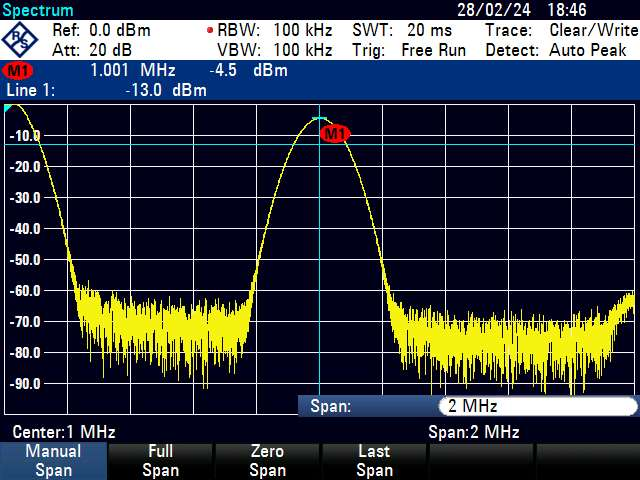
\includegraphics[width=292px]{q2_2.png}
        \caption{Estudi de la forma del primer harmònic}
        \label{fig:q2}
    \end{center}
\end{figure}

\newthought{Activitat 1.4} El senyal mostrat per pantalla és pràcticament una recta. El SA no fa cap mena d'escombrat només avaluem una freqüència. La traça baixa ràpidament quan movem la freqüència central.

\newthought{Activitat 1.5} El millor que es pot fer és baixar l'amplada de banda del filtre de vídeo per eliminar soroll, posar a \qty{0}{\deci\bel} l'atenuació, i pujar una mica l'amplada de banda del filtre estàtic. Tot i això, no he estat capaç de veure el tercer harmònic. Veure la figura \ref{fig:q3}.

\begin{figure}
    \begin{center}
        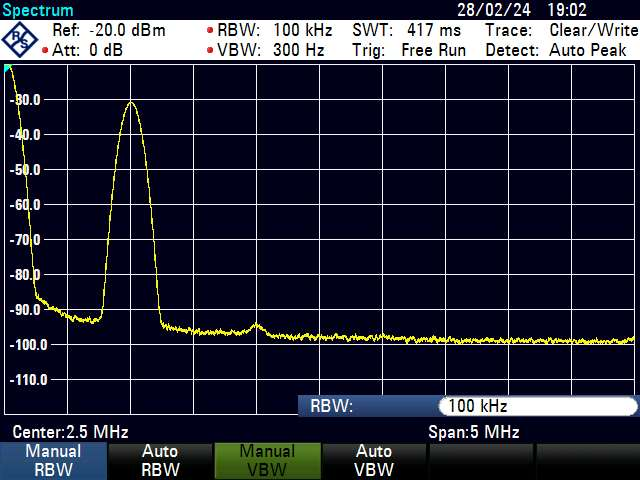
\includegraphics[width=292px]{q3.png}
        \caption{Mesura d'una senyal de baixa potència}
        \label{fig:q3}
    \end{center}
\end{figure}

\newpage

\newthought{Qüestió 1.2} Si el GF està configurat per proporcionar una amplitud \qty{200}{\milli\volt} en circuit obert, amb una càrrega de $R_L=\qty{50}{\ohm}$ proporcionarà una amplitud $v_o=\qty{100}{\milli\volt}$. El voltatge efectiu serà $\hat{v_o}=\frac{v_o}{\sqrt{2}}\simeq\qty{70.7}{\milli\volt}$. La potència mitjana és $\hat{P}=\frac{\left(\frac{\hat{v_o}}{\sqrt{2}}\right)^2}{R}\simeq\qty{0.1}{\milli\watt}$. En \unit[qualifier-mode = combine]{\deci\bel\of{m}} queda $P=10\log\hat{P}\simeq\qty[qualifier-mode = combine]{-10}{\deci\bel\of{m}}$.

\begin{marginfigure}
    \begin{center}
      \begin{circuitikz}[american voltages]
        \draw (0,0) to[short, o-] ++(-1.5,0) to[R=$R_G$] ++(-1.5,0) to[short] ++(-0.5,0) to[V=$V_G$] ++(0,-2) to[short, -o] ++(3.5,0);
        \draw (0,0) to[open, v^>=$V_o$] ++(0,-2);
        \draw (-1,0) to[R=$R_L$] ++(0,-2);
      \end{circuitikz}
    \end{center}
    \caption{Circuit equivalent del generador amb càrrega}
    \label{fig:qe2}
\end{marginfigure}

\end{document}